\documentclass[aspectratio=169]{beamer}

\usepackage[utf8]{inputenc}
\usepackage{array}
\usepackage{booktabs}
\usepackage{bold-extra}
\usepackage{graphics}
\usepackage{hyperref}
\hypersetup{%
  colorlinks=true,
  linkcolor=blue,
  filecolor=blue,
  urlcolor=cyan,
}
\usepackage{listings}
\usepackage{multicol}
\usepackage{multirow}
\usepackage[absolute,overlay]{textpos}
\usepackage{setspace}
\usepackage{verbatim}
\usepackage{fancyvrb} % for verbatim centering
\usepackage{tikz}

\usetheme{Warsaw}
\usecolortheme{beaver}
\definecolor{clOrange}{HTML}{E76600}
\definecolor{clAlmostWhite}{HTML}{FEFFD9}
\definecolor{clGreen}{HTML}{007F00}
\definecolor{clFlag}{HTML}{D33682}
\definecolor{clFlagOpt}{HTML}{CB4B16}
\definecolor{clRedFlag}{HTML}{DC322F}
\definecolor{clViolet}{HTML}{4c0070}

\definecolor{clCodeBlue}{rgb}{0.0, 0.18, 0.38}
\definecolor{clCodeGreen}{rgb}{0.0, 0.27, 0.15}
\definecolor{clCodeRed}{rgb}{0.63, 0.0, 0.0}

% A 12-bit rainbow color palette easy on the eyes, from https://iamkate.com/data/12-bit-rainbow/ :
\definecolor{clTwelveBitPink}{HTML}{881177}
\definecolor{clTwelveBitRed}{HTML}{AA3355}
\definecolor{clTwelveBitLightRed}{HTML}{CC6666}
\definecolor{clTwelveBitOrange}{HTML}{EE9944}
\definecolor{clTwelveBitYellow}{HTML}{EEDD00}
\definecolor{clTwelveBitLightGreen}{HTML}{99DD55}
\definecolor{clTwelveBitGreen}{HTML}{44DD88}
\definecolor{clTwelveBitAqua}{HTML}{22CCBB}
\definecolor{clTwelveBitCyan}{HTML}{00BBCC}
\definecolor{clTwelveBitBlue}{HTML}{0099CC}
\definecolor{clTwelveBitNavy}{HTML}{3366BB}
\definecolor{clTwelveBitViolet}{HTML}{663399}
\definecolor{clTwelveBitDarkGray}{HTML}{444444}
\definecolor{clTwelveBitLightGray}{HTML}{888888}

\setbeamertemplate{navigation symbols}{}
\setbeamercolor{title}{fg=black}
\setbeamercolor{author}{fg=clAlmostWhite}
\setbeamercolor{date}{fg=clAlmostWhite}
\setbeamerfont{author}{size=\huge}
\setbeamerfont{date}{size=\Large}

\newcommand{\greenemph}[1]{\textit{\textcolor{clGreen}{#1}}}
\newcommand{\cpp}[1]{\texttt{\textbf{\textcolor{clCodeBlue}{#1}}}}

\newcommand\fontV{\fontsize{5}{5}\selectfont}

\lstset{
  language=C++,
  basicstyle=\ttfamily,
  keywordstyle=\color{clCodeBlue}\ttfamily,
  stringstyle=\color{clCodeGreen}\ttfamily,
  commentstyle=\color{clCodeRed}\ttfamily,
  morecomment=[l][\color{magenta}]{\#}
}

\title[Friends\#25 :: \cpp{Random}]{Generating random values in modern \cpp{C++}}
\author{Adam Graliński}
\date[Dec'22]{\textbf{\texttt{\color[HTML]{d33682}C++} {\color[HTML]{268bd2}F}{\color[HTML]{2aa198}r}{\color[HTML]{859900}i}%
{\color[HTML]{cb4b16}e}{\color[HTML]{dc322f}n}{\color[HTML]{6c71c4}d}{\color[HTML]{b58900}s}, December 2022}}

\begin{document}

{\usebackgroundtemplate{%
 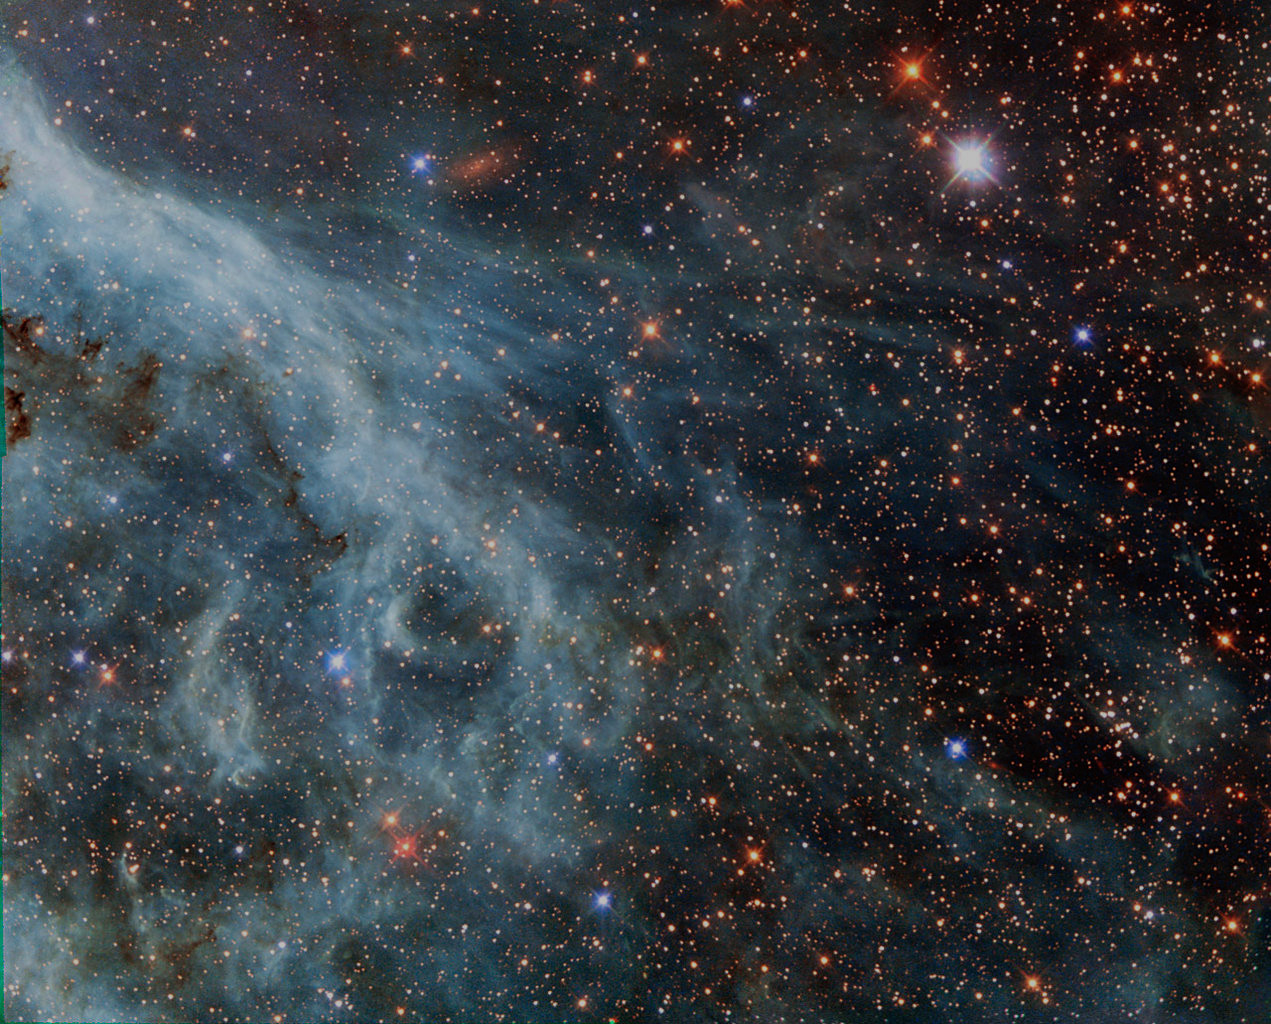
\includegraphics[width=\paperwidth,height=\paperheight]{../common/bg_galaxy.jpg}}
\begin{frame}
\titlepage{}
\end{frame}
}

\begin{frame}[fragile]
\frametitle{The common basics}
    \texttt{\textcolor{clTwelveBitLightGray}{\#include} \textbf{\textcolor{clTwelveBitDarkGray}{<random>}}}\\
    \texttt{\textit{\textcolor{clTwelveBitCyan}{random\_engine\_type}} \textcolor{clTwelveBitOrange}{engine} \{seed\};}\\
    \texttt{\textit{\textcolor{clTwelveBitCyan}{distribution\_type}} \textcolor{clTwelveBitLightGreen}{distribution} \textcolor{clTwelveBitLightGray}{\{params\};}}\\
    \texttt{\textit{\textcolor{clTwelveBitLightGray}{auto}} \textcolor{clTwelveBitViolet}{random\_value} =
        \textcolor{clTwelveBitLightGreen}{distribution}(\textcolor{clTwelveBitOrange}{engine});}\\
\end{frame}

\begin{frame}[fragile]
\frametitle{Generating uniformly random numbers}
  {\Large Task 1, ``\textit{tossing a fair dice}''}\\
  \vspace{12pt}
  Generate 10 random integers in range $\{0-9\}$.\\
  Then, generate 5 random doubles in range $[-2 - 3.4567)$.\\
\end{frame}

\begin{frame}[fragile]
\frametitle{Generating uniformly random numbers}
\begin{columns}[T]
  \begin{column}{0.6\textwidth}<1->
    {\color[HTML]{cb4b16}
    \texttt{\textbf{uniform\_random\_numbers.cpp}}\vspace{-9pt}
    \rule{\linewidth}{2pt}}%
    {\fontsize{7}{6} \lstinputlisting[showstringspaces=false]{code/uniform_random_numbers.cpp}}%
    \vspace{-12pt}{\color[HTML]{cb4b16}\rule{\linewidth}{2pt}}%
  \end{column}
  \begin{column}{0.3\textwidth}<2->
    {\color[HTML]{002b36}
    \texttt{\textbf{output}}\vspace{-9pt}
    \rule{\linewidth}{2pt}}%
    {\fontsize{8}{6} \begin{lstlisting}[showstringspaces=false]
9 5 8 5 2 5 3 5 0 6
-0.884833 -0.33921 -0.931109
1.73953 -1.92783
    \end{lstlisting}}
    \vspace{-12pt}{\color[HTML]{002b36}\rule{\linewidth}{2pt}}%
  \end{column}
\end{columns}
\pause{}
\begin{center}\url{https://godbolt.org/z/nWf3n3xdT}\end{center}
\end{frame}


\begin{frame}[fragile]
\frametitle{Generating skewed booleans}
  {\Large Task 2, ``\textit{flipping a weighted coin}''}\\
  \vspace{12pt}
  Generate 10 random boolean values, each having 40\% chance of being \cpp{true}.
\end{frame}


\begin{frame}[fragile]
\frametitle{Generating skewed booleans}
\begin{columns}[T]
  \begin{column}{0.6\textwidth}<1->
    {\color[HTML]{cb4b16}
    \texttt{\textbf{coin\_flip.cpp}}\vspace{-9pt}
    \rule{\linewidth}{2pt}}%
    {\fontsize{8}{6} \lstinputlisting[showstringspaces=false]{code/coin_flip.cpp}}%
    \vspace{-12pt}{\color[HTML]{cb4b16}\rule{\linewidth}{2pt}}%
  \end{column}
  \begin{column}{0.3\textwidth}<2->
    {\color[HTML]{002b36}
    \texttt{\textbf{possible outputs}}\vspace{-9pt}
    \rule{\linewidth}{2pt}}%
    {\fontsize{8}{6} \begin{lstlisting}[showstringspaces=false]
H H T T T H T T T T 

T T H H T H H T T T 

T H T H H T T H H T 
    \end{lstlisting}}
    \vspace{-12pt}{\color[HTML]{002b36}\rule{\linewidth}{2pt}}%
  \end{column}
\end{columns}
\pause{}
\begin{center}\url{https://godbolt.org/z/461x4cM6W}\end{center}
\end{frame}


\begin{frame}[fragile]
\frametitle{Generating normally-distributed doubles}
  {\Large Task 3, ``\textit{generating normally-distributed double values}''}\\
  \vspace{12pt}
  Generate 20 random doubles, whose values follow normal distribution\\
  centered around $\mu{} = 10$ with standard deviation $\sigma{} = 0.5$.\\
  \vspace{24pt}
  Note: the general form of probability density function is
  $$f(x) = \frac{1}{\sigma\sqrt{2\pi}}e^{-0.5(\frac{x-\mu}{\sigma})^2}$$
\end{frame}


\begin{frame}[fragile]
\frametitle{Generating normally-distributed doubles}
\begin{columns}[T]
  \begin{column}{0.6\textwidth}<1->
    {\color[HTML]{cb4b16}
    \texttt{\textbf{normal.cpp}}\vspace{-9pt}
    \rule{\linewidth}{2pt}}%
    {\fontsize{8}{6} \lstinputlisting[showstringspaces=false]{code/normal.cpp}}%
    \vspace{-12pt}{\color[HTML]{cb4b16}\rule{\linewidth}{2pt}}%
  \end{column}
  \begin{column}{0.3\textwidth}<2->
    {\color[HTML]{002b36}
    \texttt{\textbf{possible output}}\vspace{-9pt}
    \rule{\linewidth}{2pt}}%
    {\fontsize{8}{6} \begin{lstlisting}[showstringspaces=false]
9.810
9.747
9.527
9.268
9.318
9.751
9.890
9.850
10.452
10.277
10.834
10.379
10.014
10.875
10.549
9.890
10.235
10.243
10.400
9.711
    \end{lstlisting}}
    \vspace{-12pt}{\color[HTML]{002b36}\rule{\linewidth}{2pt}}%
  \end{column}
\end{columns}
\pause{}
\begin{center}\url{https://godbolt.org/z/MGzxhv4qY}\end{center}
\end{frame}



\begin{frame}
\frametitle{Key takeaways}
{\centering
\begin{itemize}
  \item{} Random numbers are generated by distributions
  \item{} Distributions utilize \textit{uniform random bit engines}.
  \item{} No single global state. Many random engines can coexist independently.
  \item{} Nice properties, \textit{fast}, but not cryptographically secure
  \begin{itemize}
    \item{} CSPRNG still not standardized in \cpp{C++}
    \item{} tap \cpp{/dev/urandom} on most *nix systems,\\
            use \cpp{CryptGenRandom} on Windows, \cpp{getentropy} on OpenBSD
    \item{} there's also \cpp{boost::random\_device} - a true CSPRNG. Portable and well tested.
  \end{itemize}

\end{itemize}

\vspace{2ex}
\begin{center}{\Large Thank you!}\end{center}
}
\end{frame}

%%%%

\end{document}
